\subsection{Syntax units}
\label{sec:syntax-units}

\begin{figure*}[t]
    \begin{subfigure}{0.32\textwidth}
            \centering
            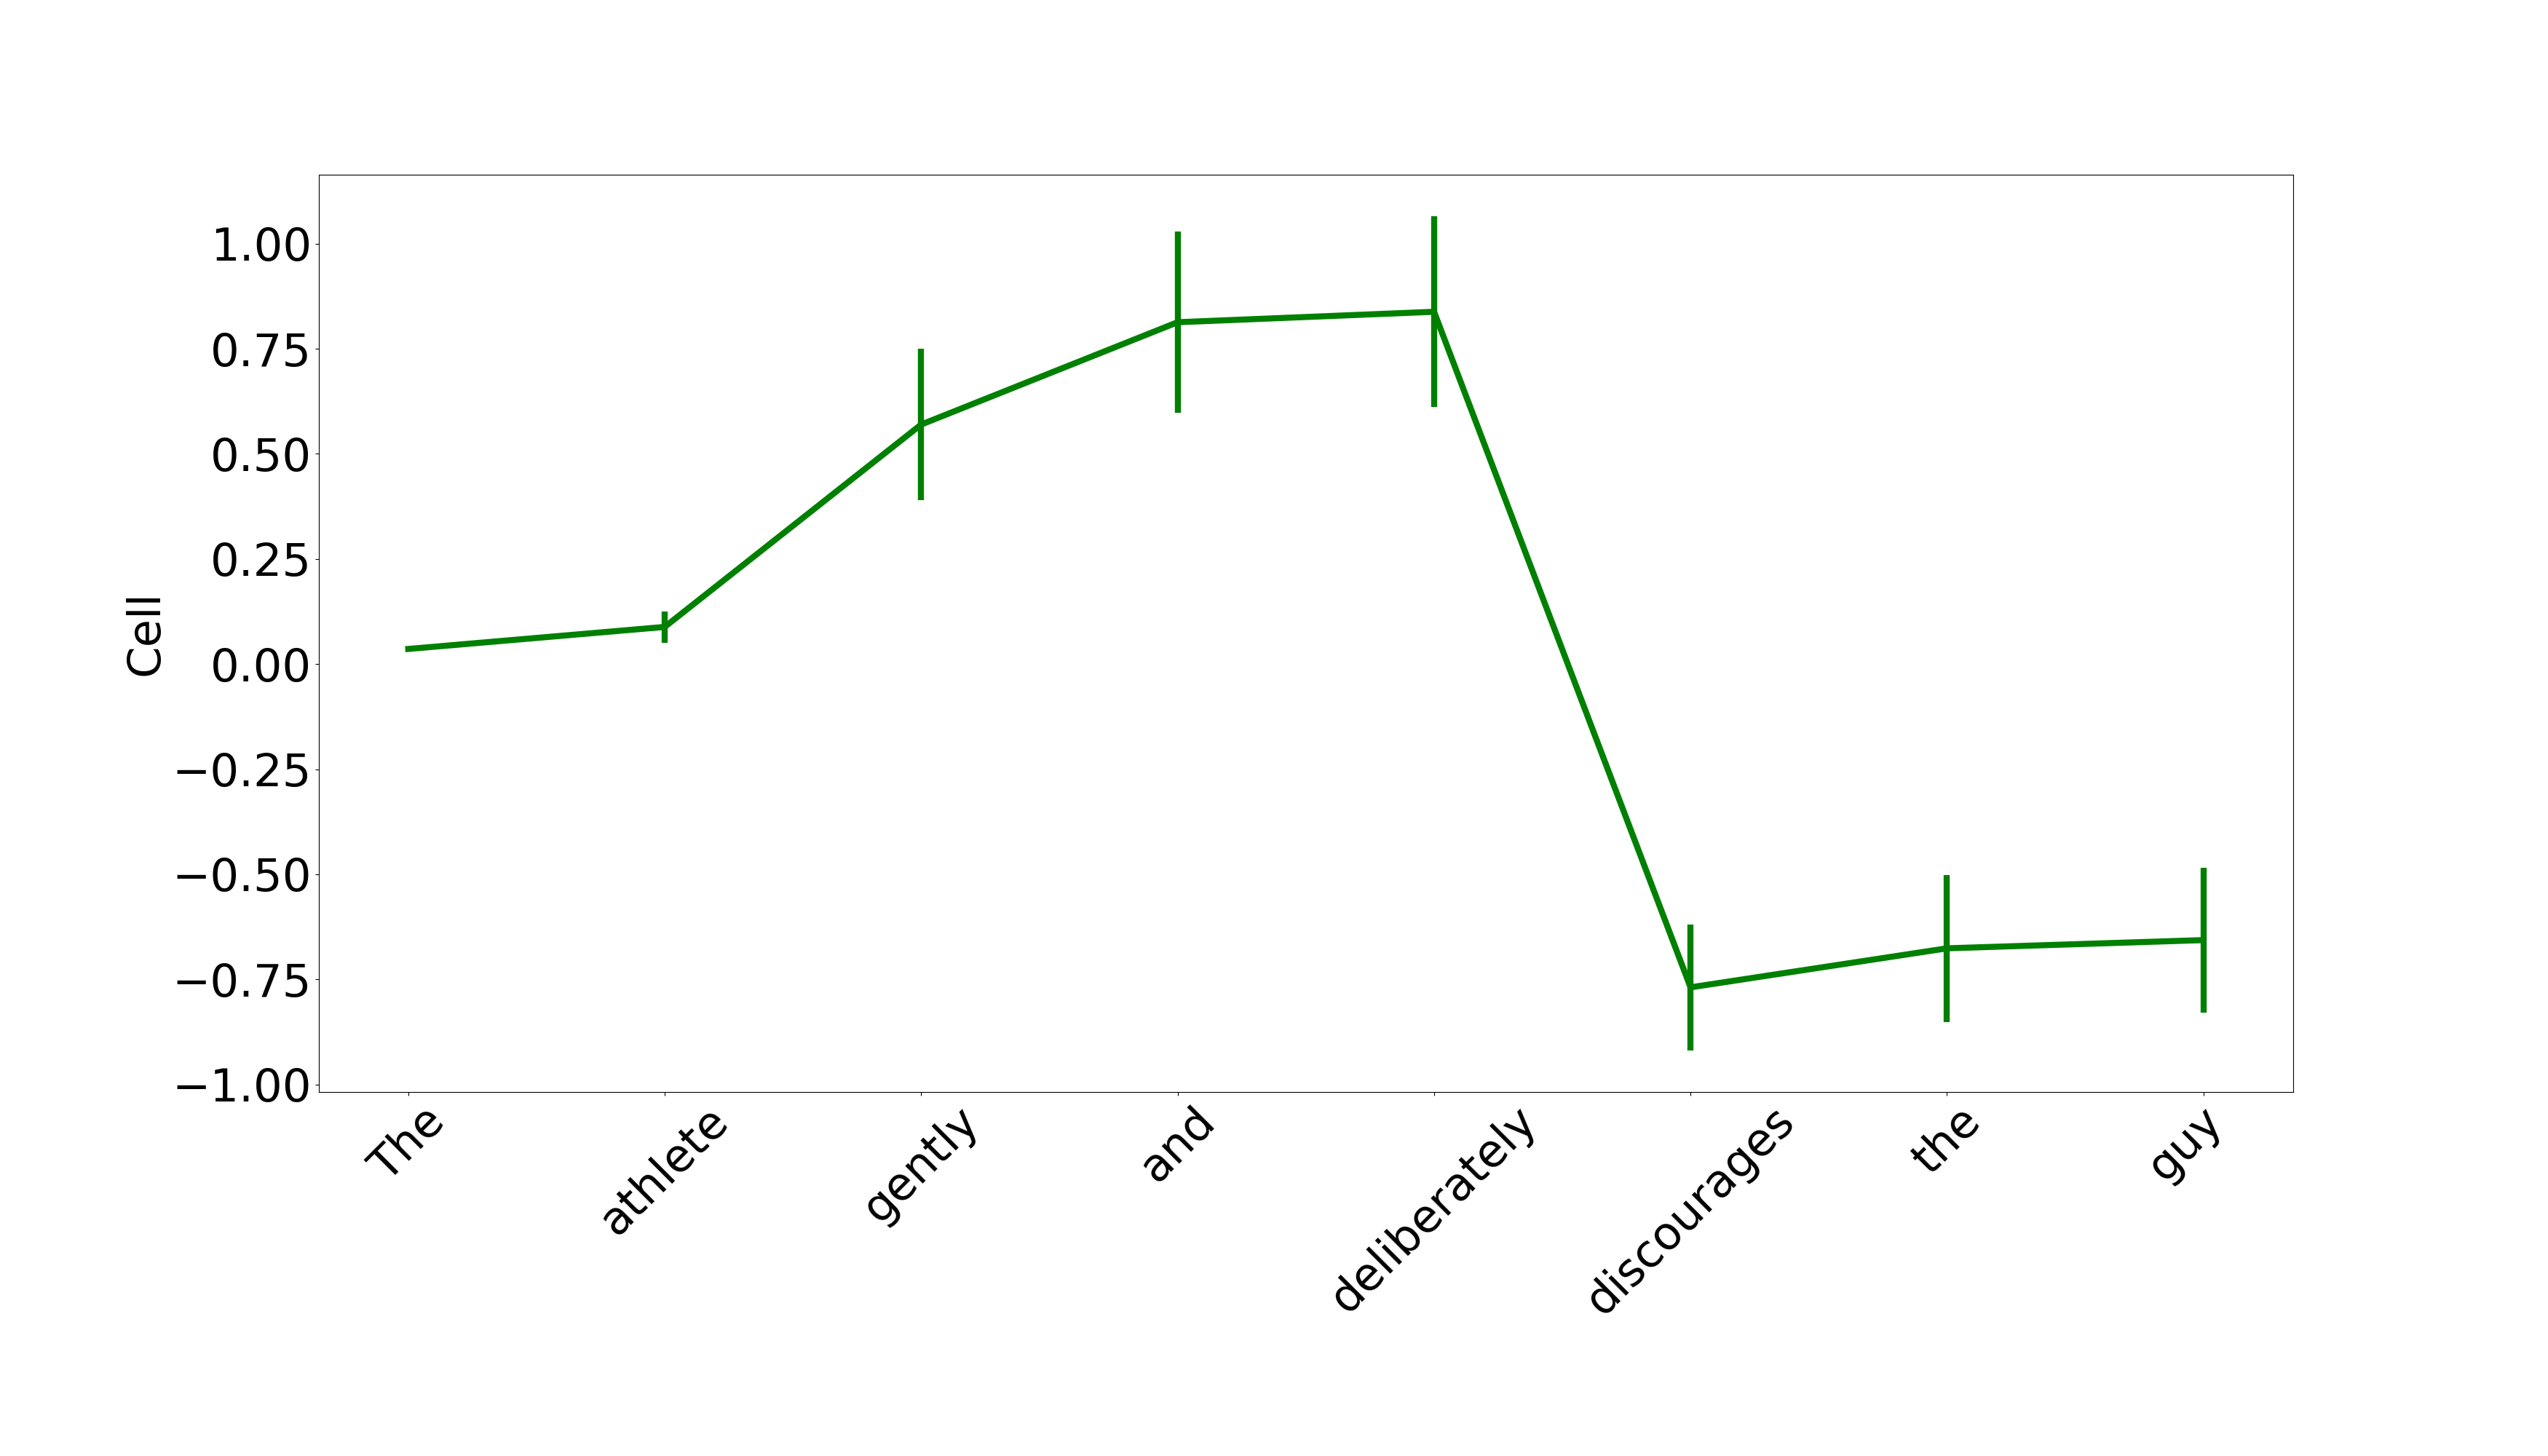
\includegraphics[width=\linewidth, height=1.9cm]{Figures/adv_conjunction_1149_cell}
            \caption{2Adv}
            \label{fig:syntax-unit-2Adv}
    \end{subfigure}
    \begin{subfigure}{0.32\textwidth}
            \centering
            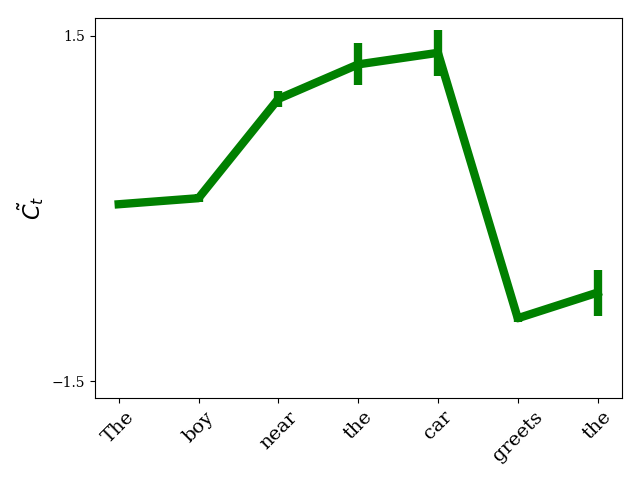
\includegraphics[width=\linewidth, height=1.9cm]{Figures/nounpp_1149_cell.png}
            \caption{nounPP}
            \label{fig:syntax-unit-nounpp}
    \end{subfigure}
    \begin{subfigure}{0.32\textwidth}
            \centering
            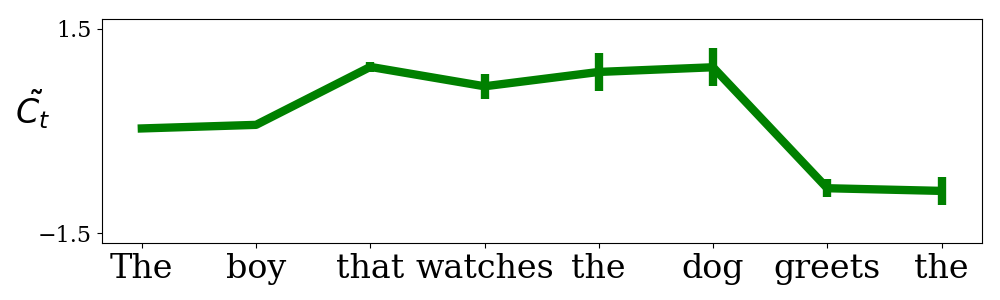
\includegraphics[width=\linewidth, height=1.9cm]{Figures/subjrel_that_1149_cell.png}
            \caption{subject relative}
            \label{fig:syntax-unit-subjrel}
    \end{subfigure}
    \begin{subfigure}{\textwidth}
            \centering
            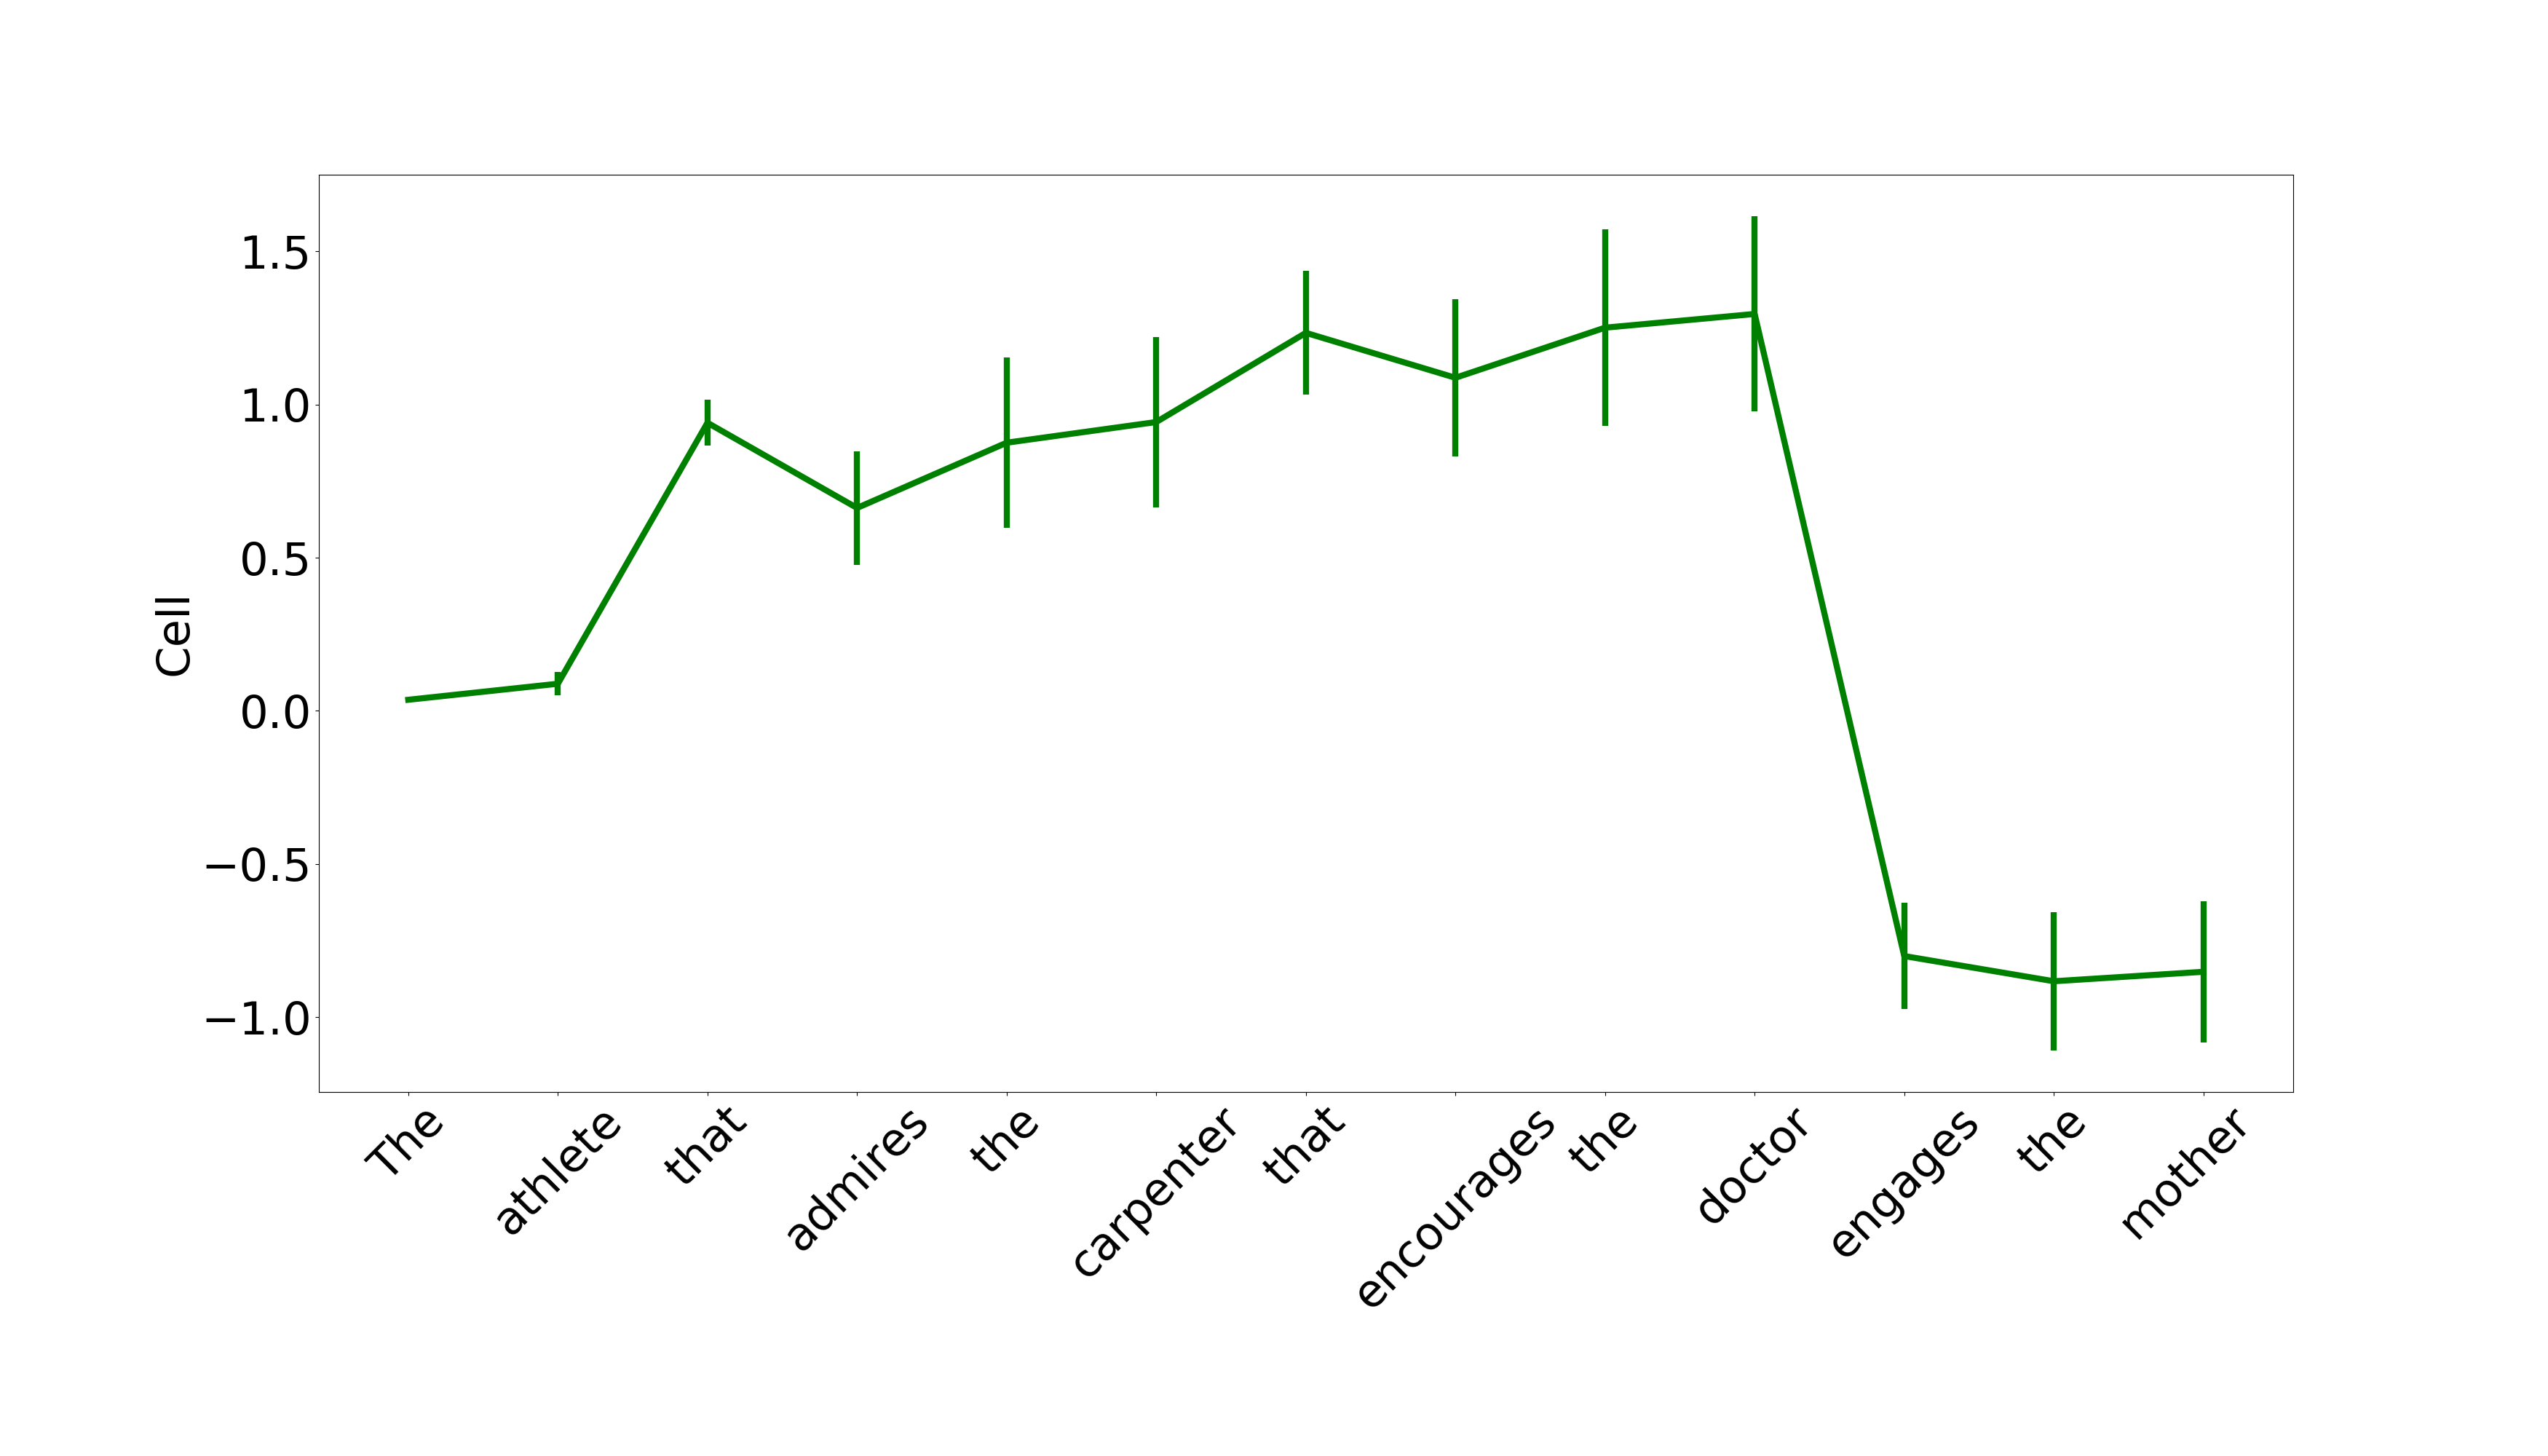
\includegraphics[width=\linewidth, height=2cm]{Figures/double_subjrel_that_1149_cell.png}
            \caption{Two embeddings with subject relatives}
            \label{fig:syntax-unit-double-subjrel}
    \end{subfigure}
\caption{Cell activity of syntax unit \unit{2}{500} while processing various syntactic structures. Values averaged across all stimuli in an NA-task, with error bars representing standard deviations. Relative clause NA-task stimuli were specifically generated for this visualization.}
\end{figure*}

We saw how the input and forget gates of the LR-number units control the flow
of subject-number information. It remains unclear, however, how the dynamics of these gates are controlled by the network. We hypothesized
that other units may encode information about the syntactic structure
of the sentence, and thus about the subject-verb dependency. To
search for them, we tested whether syntactic information can be
decoded from some network units, by using depth of the
syntactic tree as a proxy \cite{Nelson:etal:2017}. Specifically, we
trained an L2-regularized regression model to predict syntactic
tree-depth from the hidden-state activity of all units, using the data
presented in Section \ref{sec:the_data} above, in a nested 5-fold
cross-validation procedure. %
% (the optimal regularization size was found to be consistent across CV-splits, $\lambda=784.76$, among 20 possible values log-uniformly distributed in $[10^-5, 10^5]$). Word position and tree-depth were decorrelated in the data and
Word frequency was added as a covariate
to the model, and had a negligible effect on the results.

Syntactic tree-depth can be efficiently decoded from network activity
($R^2_{test-set}=0.85\pm0.009$; covariate-corrected). A small subset of `syntax' units had relatively high weights in the regression model (mean weight = $7.6\times{}10^{-4}$, SD=$7.86\times{}10^{-2}$; cutoff for outlier weights was set to three SDs). Since the interpretation of the regression weights may depend on possible correlations among the features, we also tested the causal effect of these units on NA-task performance. Ablating the syntax units together resulted in significant performance reduction in NA-tasks that have an interfering noun: Linzen NA-task: $p=0.024$, nounPPAdv-SP: $p=0.011$, nounPPAdv-PS: $p=0.034$, nounPP-SP: $p<0.001$ and marginally significant in nounPP-PS: $p=0.052$ (compared to 1000 random ablations of subsets of units of the same size).

To gain further insight regarding the functioning of the syntax units,
we next visualized their gate and cell dynamics during sentence
processing. We found that cell activity of unit
\unit{2}{500}, which also had one of the highest weights in the
regression model, was remarkably structured. The activity of
this unit increases across the entire subject-verb
dependency and drops abruptly right after. Figures
\ref{fig:syntax-unit-2Adv} and \ref{fig:syntax-unit-nounpp} show cell
activity of this unit during the processing of stimuli from the 2Adv
and nounPP tasks. We found the same dynamics in cases where another
verb occurs between subject and main verb, as in subject relatives
(Figure \ref{fig:syntax-unit-subjrel}), and in exceptionally
long-distance dependencies with two interfering nouns and verbs
(Figure \ref{fig:syntax-unit-double-subjrel}). Taken together, these
results suggest that unit \unit{2}{500} consistently encodes
subject-verb dependency in a syntax-sensitive manner. Other syntax
units did not show an easily interpretable dynamics, and had no clear
interactions with the number units in the analysis discussed next,
suggesting that they perform different syntactic, or possibly other, functions.